% 2010 年天津卷理科第 14 题：圆内接四边形 ABCD 与两割线交点 P。
% 来源 PDF：普通高考/2010/2010天津理.pdf，SHA-256 340aba76699a12f330637f9c682abbc893e03e0e91788287934c0a7e0a3cace9。
% 原页：第 1 页（A3 六栏）第 3 栏上部，书页码 635。
% 重绘依据：A、B、C、D 依次在圆上；P 为 AB 与 DC 延长线的交点，
%   连线 A—B—P 与 D—C—P 为割线，另画弦 AD 与弦 BC。
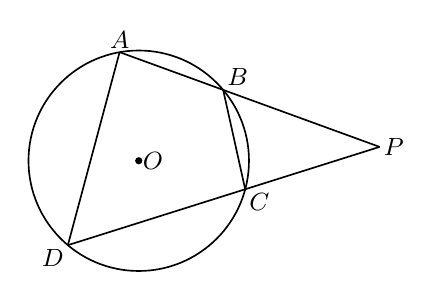
\begin{tikzpicture}[semithick, every node/.style={inner sep=1.2pt, font=\small}]
  \coordinate (O) at (0,0);
  \coordinate (A) at (-0.243,1.379);
  \coordinate (B) at (1.072,0.900);
  \coordinate (C) at (1.352,-0.362);
  \coordinate (D) at (-0.900,-1.072);
  \coordinate (P) at (3.059,0.176);
  \draw (0,0) circle (1.4);
  \fill (O) circle (1.3pt);
  \draw (A) -- (P);
  \draw (D) -- (P);
  \draw (A) -- (D);
  \draw (B) -- (C);
  \node[above] at (A) {$A$};
  \node[above right] at (B) {$B$};
  \node[below right] at (C) {$C$};
  \node[below left] at (D) {$D$};
  \node[right] at (P) {$P$};
  \node[right] at (O) {$O$};
\end{tikzpicture}
